\section{Introduction to JML on a Example}
\label{sec-RunningExample}


\begin{floatingfigure}[l]{6cm}
\begin{center}
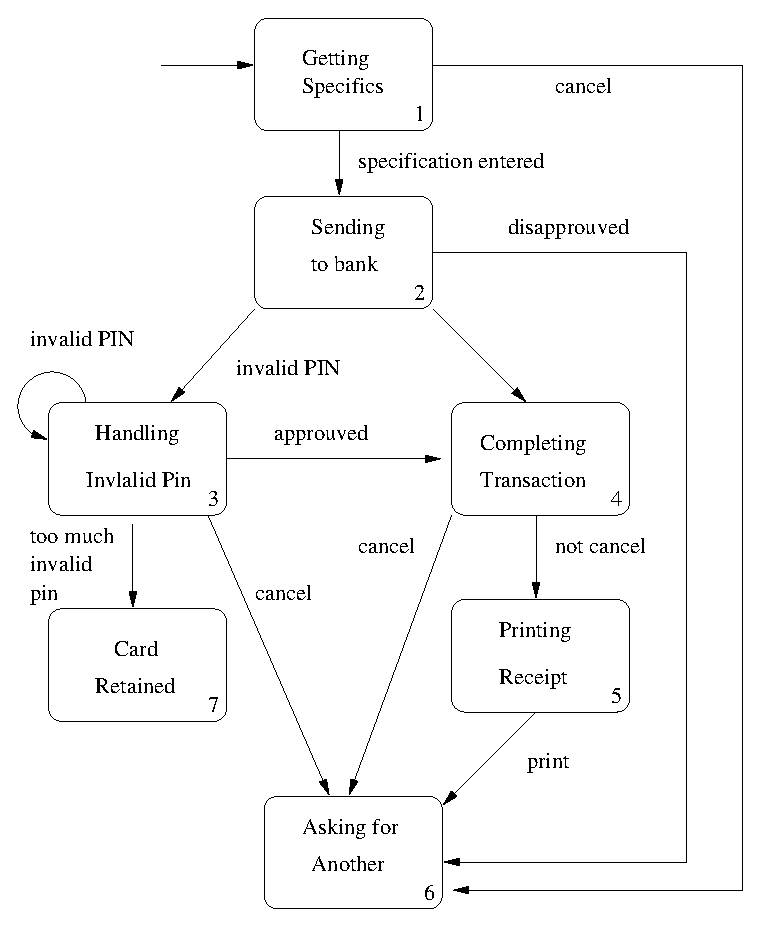
\includegraphics[scale=0.4]{Transac.eps}
\end{center}
\caption{Transaction System Graph}
\label{fig-Transac}
\end{floatingfigure}
The transaction mechanism of 
the ATM specification (see Sect.~\ref{SecIntro}) 
was initially designed by a 
 diagram (see Fig.~\ref{fig-Transac}). It works as follows.
First, when a transaction is initialized, it get information
from the customer (amount, type of transaction...). Second,
this information is sent to the bank, which may approve 
or disapprove the transaction (amount too high for the account...).
In the case of approval, and if the PIN code is confirmed, the
transaction can be completed. Otherwise the PIN code is asked again
until the PIN limit (normally only three at\-tem\-pts are authorized). When
the PIN lim\-it is reached, the card is retained. 
After a transaction completion, the customer may obtain a ticket. 
At each step, it is possible to cancel the transaction.
%We would like to implement this transaction system. 
This transaction system is implemented by a Java Class $Transaction$.
We have 
described this class, according to the diagram (see Fig.~\ref{fig-Transac})
using JML specifications (Fig.~\ref{FigRunningExample}).
JML (Java Modeling
Language)~\cite{Leavens-etal03} is a specification
language especially tailored for Java applications. Originally, JML
was proposed by G.T.~Lea\-vens and his team; nowadays the development of
JML is a community effort. JML has been successfully used in several
case studies to specify Java applications, and notably to specify
smart card applications, written in Java
Card~\cite{BreunesseCHJ03,BousquetLMOL04,JacobsMR04}.



%%%%%%%%%%%%%%%%%%%%%%%%%%%%%%%%%%%%%%%%%%%%%%%%%%%%%%%%%%%
%JML introduce its own  variables. 
%These exist also only in specifications, but a special
%\texttt{set} annotation exists to change their value.% (while
%\texttt{model} variables change implicitly, when the concrete
%variables they represent change).
%F%urther 
The reader can see a declaration of a class \texttt{invariant}, denoting a
predicate that has to hold before and after every method call.  We can also
specify history \texttt{constraint}s, expressing a relation between the
pre- and post-state of a method. Pre-state values of expressions are
denoted by the JML keyword \texttt{$\backslash$old}. Moreover, one can
specify, using the clause \texttt{for}, the list of the methods on which
the history constraint must be verified. When this clause is omitted, the
constraint must hold on all the methods of the class.  Finally, behavior of
the methods can be specified using keyword \texttt{normal\_behavior}. The
clause \texttt{requires} denotes the precondition of the method, i.e.  a
predicate that must be true when the method is called. We can also specify
postcondition (\texttt{ensures} clause).  A method can terminate
exceptionally, by throwing an exception and satisfying the exceptional
postcondition (\texttt{signals} clause). In this case, we have a
\texttt{behavior} specification. The validation of this model can be done
using JML-TT-Animator, a symbolic animator for JML
specification~\cite{bdlu05}. The faithfulness of the JML model w.r.t. the
Java code is done by a prover (B or Coq) via a proof
obligations generator (Jack or Krakatoa). 
 


In the rest of the paper, given the JML model of a class $C$, we denote 
\(\mathcal{P}red_C\) the set of the JML predicates.




% \marginpar{ajouter
% que la conformité à la spec n'est pas une garantie: faut-il encore que la spec n'ait pas de faille.}




\begin{figure}[h]
\begin{multicols}{2}
\begin{scriptsize}
\ttfamily

            private int state = 1;\\
            private static  int PIN\_MAX\_TRY = 3;\\
            private int pin\_try = 0;\\
           /*@ invariant state $>$= 1 \&\&\\
           ~~@ state $<$ 8;\\
           ~~@*/


            /*@ private normal\_behavior\\
~\quad         @ requires state == 1;\\
~\quad         @ modifies state;\\
~\quad         @ ensures  state == 2 \\
~\quad         @     ||  state == 6;\\
~\quad         @*/\\
            private void initialiseTransaction()\{...\}\\
           
            /*@ private  normal\_behavior\\
\quad         @ requires state == 2 ;\\
\quad         @ modifies state,pin\_try,pin\_validated;\\
\quad         @ ensures  (state == 3 \\
\quad         @ \qquad                \&\& pin\_try == $\backslash$old(pin\_try) + 1\\
\quad         @ \qquad                \&\& pin\_validated == false) \\
\quad         @ \quad     ||   (state == 6 \\
\quad         @ \qquad                \&\& pin\_try == $\backslash$old(pin\_try)\\
\quad         @ \qquad               \&\& pin\_validated == false)\\
\quad         @ \quad    ||   (state == 4 \\
\quad         @ \qquad               \&\& pin\_try == $\backslash$old(pin\_try)\\
\quad         @ \qquad               \&\& pin\_validated == true);\\
\quad         @*/\\
            private void sendToBank()\{... \}\\
            
            /*@ private behavior\\
\quad         @ requires state == 3;\\
\quad         @ modifies state,pin\_try,pin\_validated;\\
\quad         @ ensures (state == 4)\\
\quad         @  \quad     || (state == 6\\
\quad         @  \qquad         \&\& pin\_try == $\backslash$old(pin\_try)\\
\quad         @  \qquad         \&\& pin\_validated == true\\
\quad         @  \qquad         );\\
\quad         @ signals (Exception) (state == 7 \\
\quad         @  \qquad        \&\& pin\_try == PIN\_MAX\_TRY\\
\quad         @  \qquad        \&\& pin\_try == $\backslash$old(pin\_try) + 1\\
\quad         @  \qquad        \&\& pin\_validated == false);\\
\quad         @ signals (Exception) (state == 3 \\
\quad         @  \qquad        \&\& pin\_try < PIN\_MAX\_TRY\\
\quad         @  \qquad        \&\& pin\_try == $\backslash$old(pin\_try) + 1\\
\quad         @  \qquad        \&\& pin\_validated == false);\\
\quad         @*/\\
            private void pinValidation() \{... \}\\
            
            
            /*@ private  normal\_behavior\\
\quad         @ requires state == 4;\\
\quad         @ modifies state;\\
\quad         @ ensures state == 5\\
\quad         @ \qquad      || state == 6;\\
\quad         @*/\\
            private void complete()\{...\}\\
            
            
            /*@ private  normal\_behavior\\
\quad         @ requires state == 5;\\
\quad         @ modifies state;\\
\quad         @ ensures state == 6;\\
\quad         @*/\\
            private void printReceipt()\{ ... \}\\

 /*@ private  normal\_behavior\\
\quad  @ ensures $\backslash$result ==  (PIN\_MAX\_TRY - pin\_try);\\
\quad         @*/\\
public void /* pure */ getTryLess()\{...\}
          

\normalfont
\setlength{\parindent}{1cm}
\end{scriptsize}
\end{multicols}
\caption{Transaction System Example}
\label{FigRunningExample}


\end{figure}






%%% Local Variables: 
%%% mode: latex
%%% TeX-master: "main2"
%%% End: 
